\documentclass[12pt]{article}
\usepackage{amsmath}
\usepackage{graphicx}
\title{Report for Auto Control Lab7}
\date{2020/10/13}
\author{Jacky Yeh 4107064003}

\begin{document}
\begin{titlepage}

\maketitle
\end{titlepage}

\section{Introduction}
This is the fifth Experiment of Auto Control Lab where TAs taught us the plot of state transition matrix and the method of how to solve for the solution for state space variables.


\section{LAB7}
\subsection{Part 1 Homework problems and its codes}
Objective:To perform operations to find out the state space form for those certain given input,state space matrices.Also using transfer function to get state space matrices form\\

These are the stated Homework problems\\

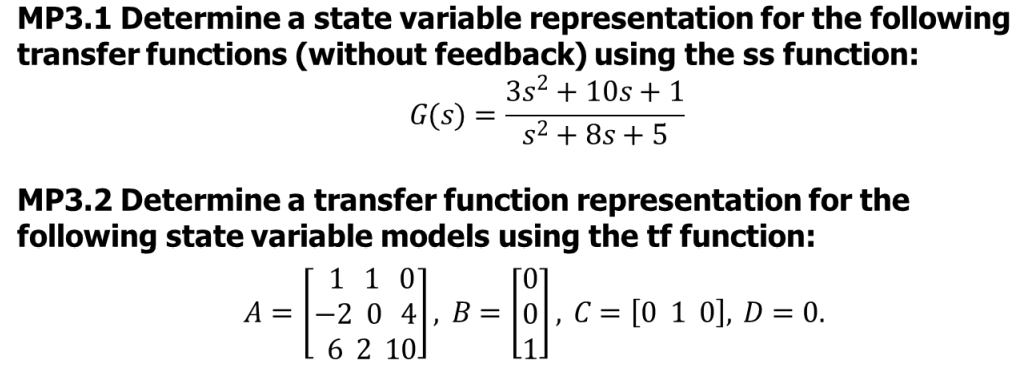
\includegraphics[scale=0.5]{HW1_problem.png} \\


\subsection{CODES FOR PROBLEM1}
In order to perform the tasks, Matlab codes are needed. The following is the code needed for generating the state space matrices and transfer function for HW problem 1 \\

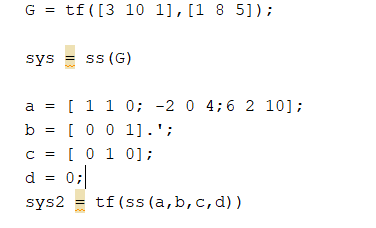
\includegraphics[scale=0.4]{HW1_problem_code.png}\\

\subsection{Result of the given state space matrices also the transformation from transfer function to state space}

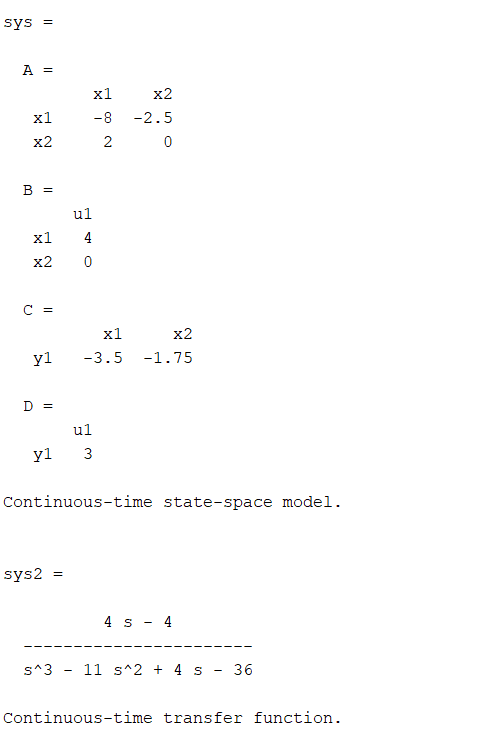
\includegraphics[scale=1]{HW1_problem_result.png}\\


\cleardoublepage




\cleardoublepage
\subsection{Part 2 Homework problems and its codes}
Objective:To plug in and plot out the response with the given system using state-space variable method. Also to find the state transition matrix also its state at a certain given time t\\
These are the stated HW problems.

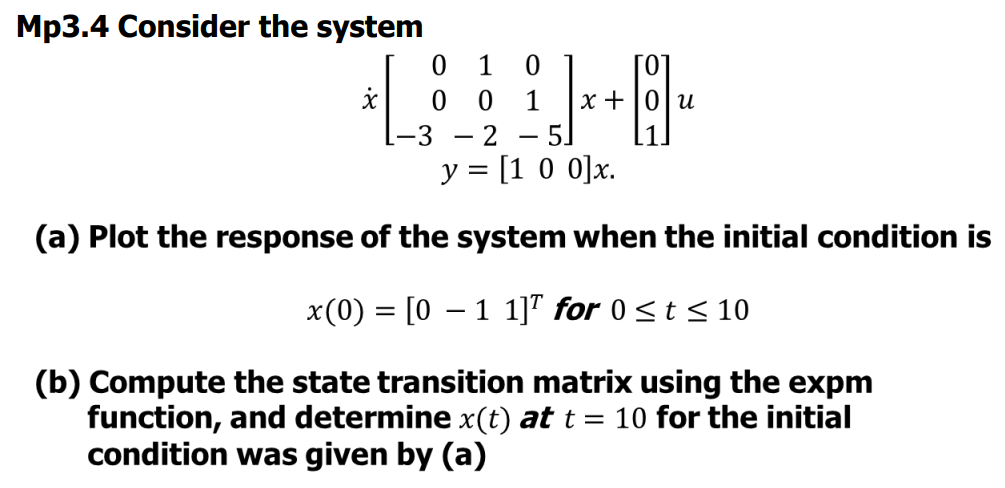
\includegraphics[scale=0.5]{HW2_problem.png} \\


\subsection{CODES FOR Part2}
In order to perform the tasks, Matlab codes are needed. The following code is used for generating the state transition matrix and finding the state output for this certain time t \\

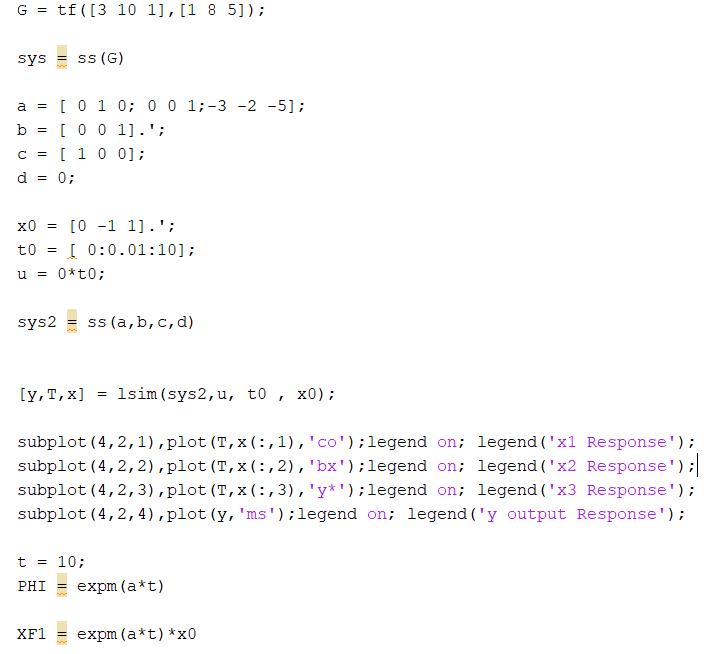
\includegraphics[scale=0.5]{HW2_code.png}
\cleardoublepage

\subsection{Plot Response OF the given system and the state transition matrix PHI}
The plot is the output at a given time t=10\\

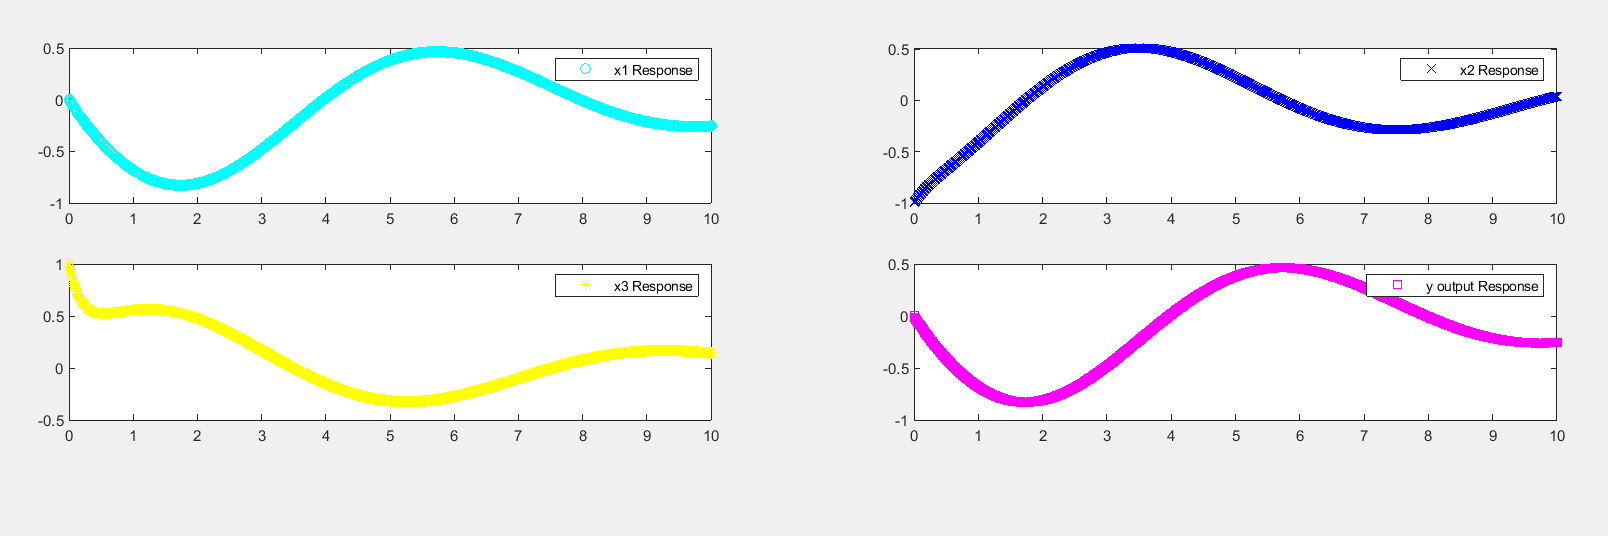
\includegraphics[scale=0.5]{HW2_code_result.png}  \\

The followings are the state transition matrix and the state given at t=10\\

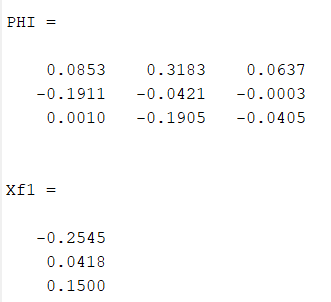
\includegraphics[scale=0.5]{HW2_problem_resultof_phi_state.png} \\


\section{Conclusion}
Today we learn how to perform operations on state-space variables to find out state-transition matrix and its output at a certain given time which is completely new for us. Today's coding experience allow us to have an even clear view about how state-space system works, instead of seeing them as Matrices A,B,C,D. Also this is an important method to search for the system output at a certain given time.This is an important topic in Auto Control.

\begin{center}
This concludes the sixth Week of Auto Control LAB\\
\end{center}

\end{document}
